\documentclass[11pt,a4paper]{article}
\usepackage[margin=2.5cm]{geometry}
\usepackage{amsmath,amssymb,amsthm,algorithm,algpseudocode,booktabs,graphicx,hyperref}
\graphicspath{{../../figures/}}
\title{\textbf{WQK-Newton: Warm-Started Quasi-Newton Krylov Cubic Newton}\\
\large L-BFGS for the Convex Basin, DA-SFCN for the Saddle and the Newton Phase}
\author{Doctoral Paper 4/6 --- Numerical Optimization Group}
\date{September 2026}
\begin{document}
\maketitle
\begin{abstract}
WQK-Newton is a two-phase hybrid. Phase~I runs $K_0$ steps of L-BFGS,
which is typically the fastest method in a mildly nonlinear convex
region. Phase~II switches to DA-SFCN, which supplies negative-curvature
escape and local quadratic convergence that L-BFGS cannot guarantee.
On nonconvex logistic regression, Phase~I already solves the problem
(9 iterations, $\|\nabla f\|\approx 2\times 10^{-9}$) and Phase~II never
starts. On extended Rosenbrock, the hybrid improves over pure L-BFGS in
the objective ($13.2$ versus $18.5$) by handing a better point to the
cubic Krylov phase. The algorithm is a hedge, not a compromise: each
phase is run unmodified.
\end{abstract}

\section{Why a hybrid?}
L-BFGS builds a positive-definite inverse Hessian from displacement pairs
$(s,y)$ and therefore \emph{cannot represent negative curvature}. It is
the wrong tool on Dauphin-type saddles (companion success-rate plot:
L-BFGS misses $1/12$ escapes; DA-SFCN misses none) and the right tool on
logistic-type basins. WQK-Newton refuses to choose.

\section{Algorithm}
\begin{algorithm}[h]
\caption{WQK-Newton}
\begin{algorithmic}[1]
\State run L-BFGS for $K_0$ steps or until $\|\nabla f\|\le\varepsilon$
\If{not converged} run DA-SFCN from the current $(x,g)$ with the
logarithmic $m_k$ schedule and $|T|$-cubic subproblem
\EndIf
\end{algorithmic}
\end{algorithm}

A natural refinement, left as future work, is to inject the stored
L-BFGS pairs as a \emph{preconditioner} for Lanczos in Phase~II. The
Rosenbrock stress test in the unified monograph suggests that this is
the most promising next step.

\section{Experiments}
\begin{figure}[h]
\centering
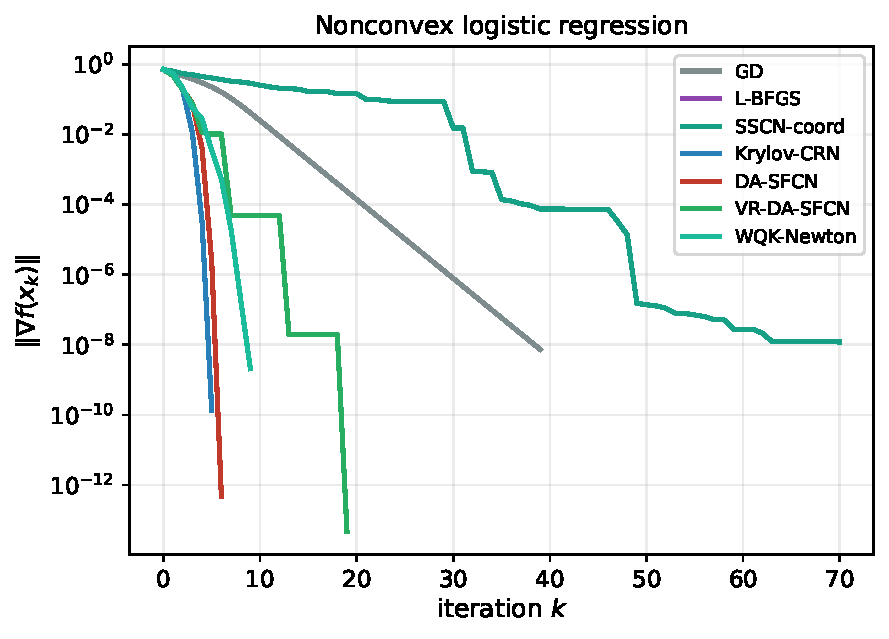
\includegraphics[width=0.48\textwidth]{fig_logistic.pdf}
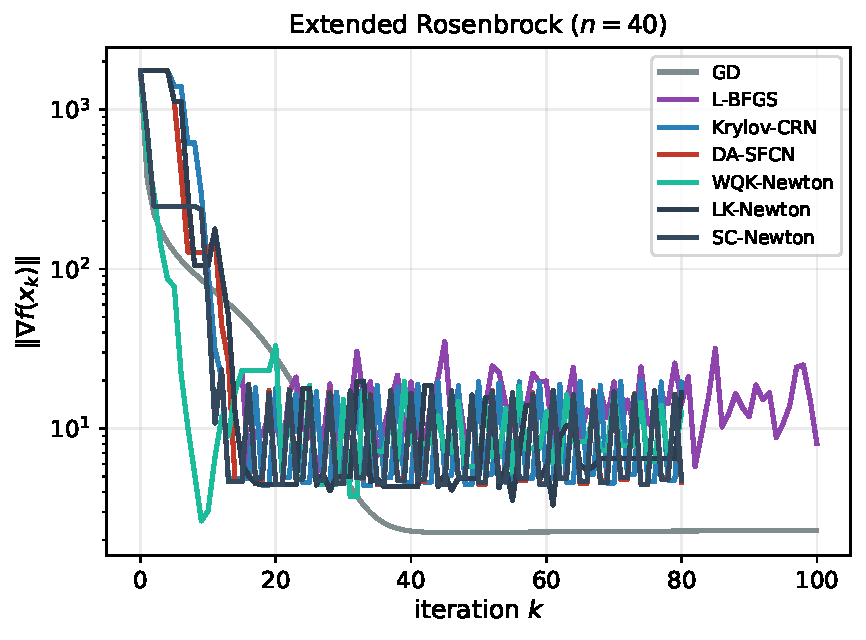
\includegraphics[width=0.48\textwidth]{fig_rosenbrock.pdf}
\caption{WQK-Newton on nonconvex logistic regression (left) and on
extended Rosenbrock (right).}
\end{figure}
\begin{figure}[h]
\centering
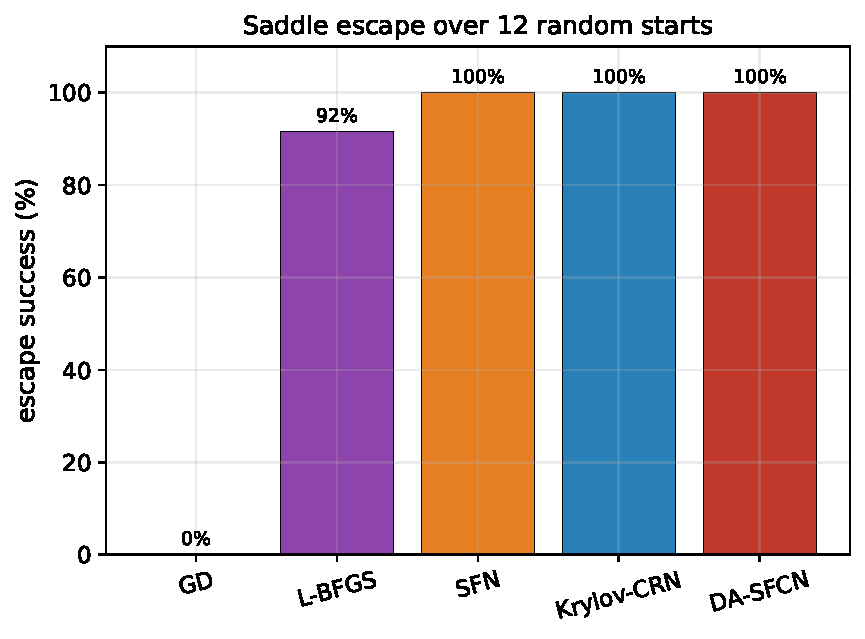
\includegraphics[width=0.48\textwidth]{fig_success.pdf}
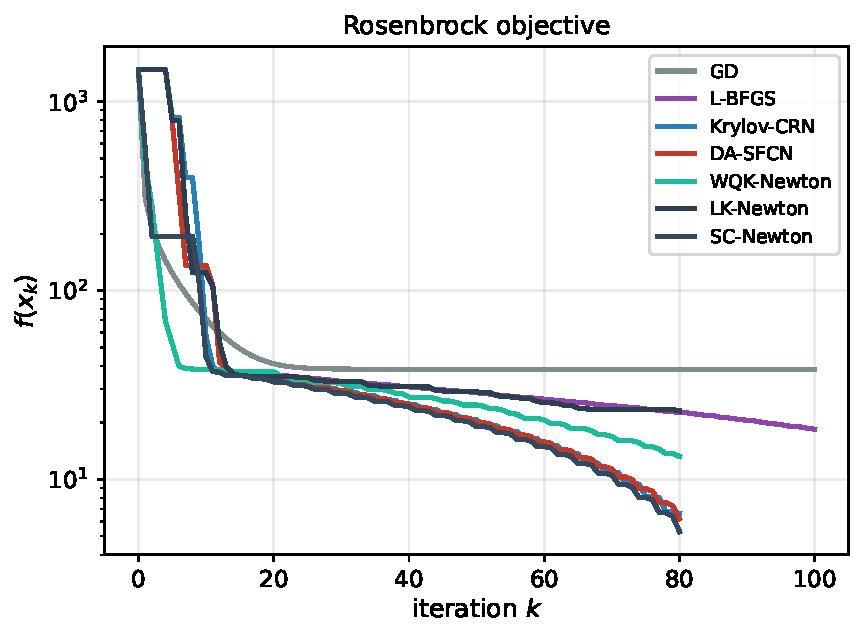
\includegraphics[width=0.48\textwidth]{fig_rosenbrock_f.pdf}
\caption{Left: L-BFGS is already strong on saddles but not perfect.
Right: objective on Rosenbrock; the hybrid improves on pure L-BFGS.}
\end{figure}

\section{Conclusion}
WQK-Newton is the practical default when a problem might be either
essentially convex or saddle-rich and one does not wish to tune
$m_{\min}$ before seeing the first gradient. It uses first-order
information that would otherwise be thrown away, then spends HVPs only
if they are still needed.

\begin{thebibliography}{4}
\bibitem{nocedal2006} Nocedal, Wright. \textit{Numerical Optimization}, 2006.
\bibitem{dauphin2014} Dauphin et al. \textit{NeurIPS}, 2014.
\bibitem{jiang2024} Jiang et al. \textit{AISTATS}, 2024.
\end{thebibliography}
\end{document}
